\documentclass{article}
\usepackage[margin=1.2in]{geometry}
\usepackage[utf8]{inputenc}
\usepackage[sharp]{easylist}
\usepackage{cite}
\usepackage{float}
\usepackage[hidelinks]{hyperref}
\usepackage{graphicx}
\usepackage{setspace}
\usepackage{amsmath}
\usepackage{caption}
\usepackage{algorithm2e}
\usepackage{pdfpages}

\setstretch{1.13}
\graphicspath{ {./figures/} }
\title{Outdoor Augmented Reality}

\begin{document}



\author{{Ethan Zammit[4802L]}\\
\textit{ethan.zammit.19@um.edu.mt}\\
\textit{University of Malta}}



\maketitle
\pagebreak
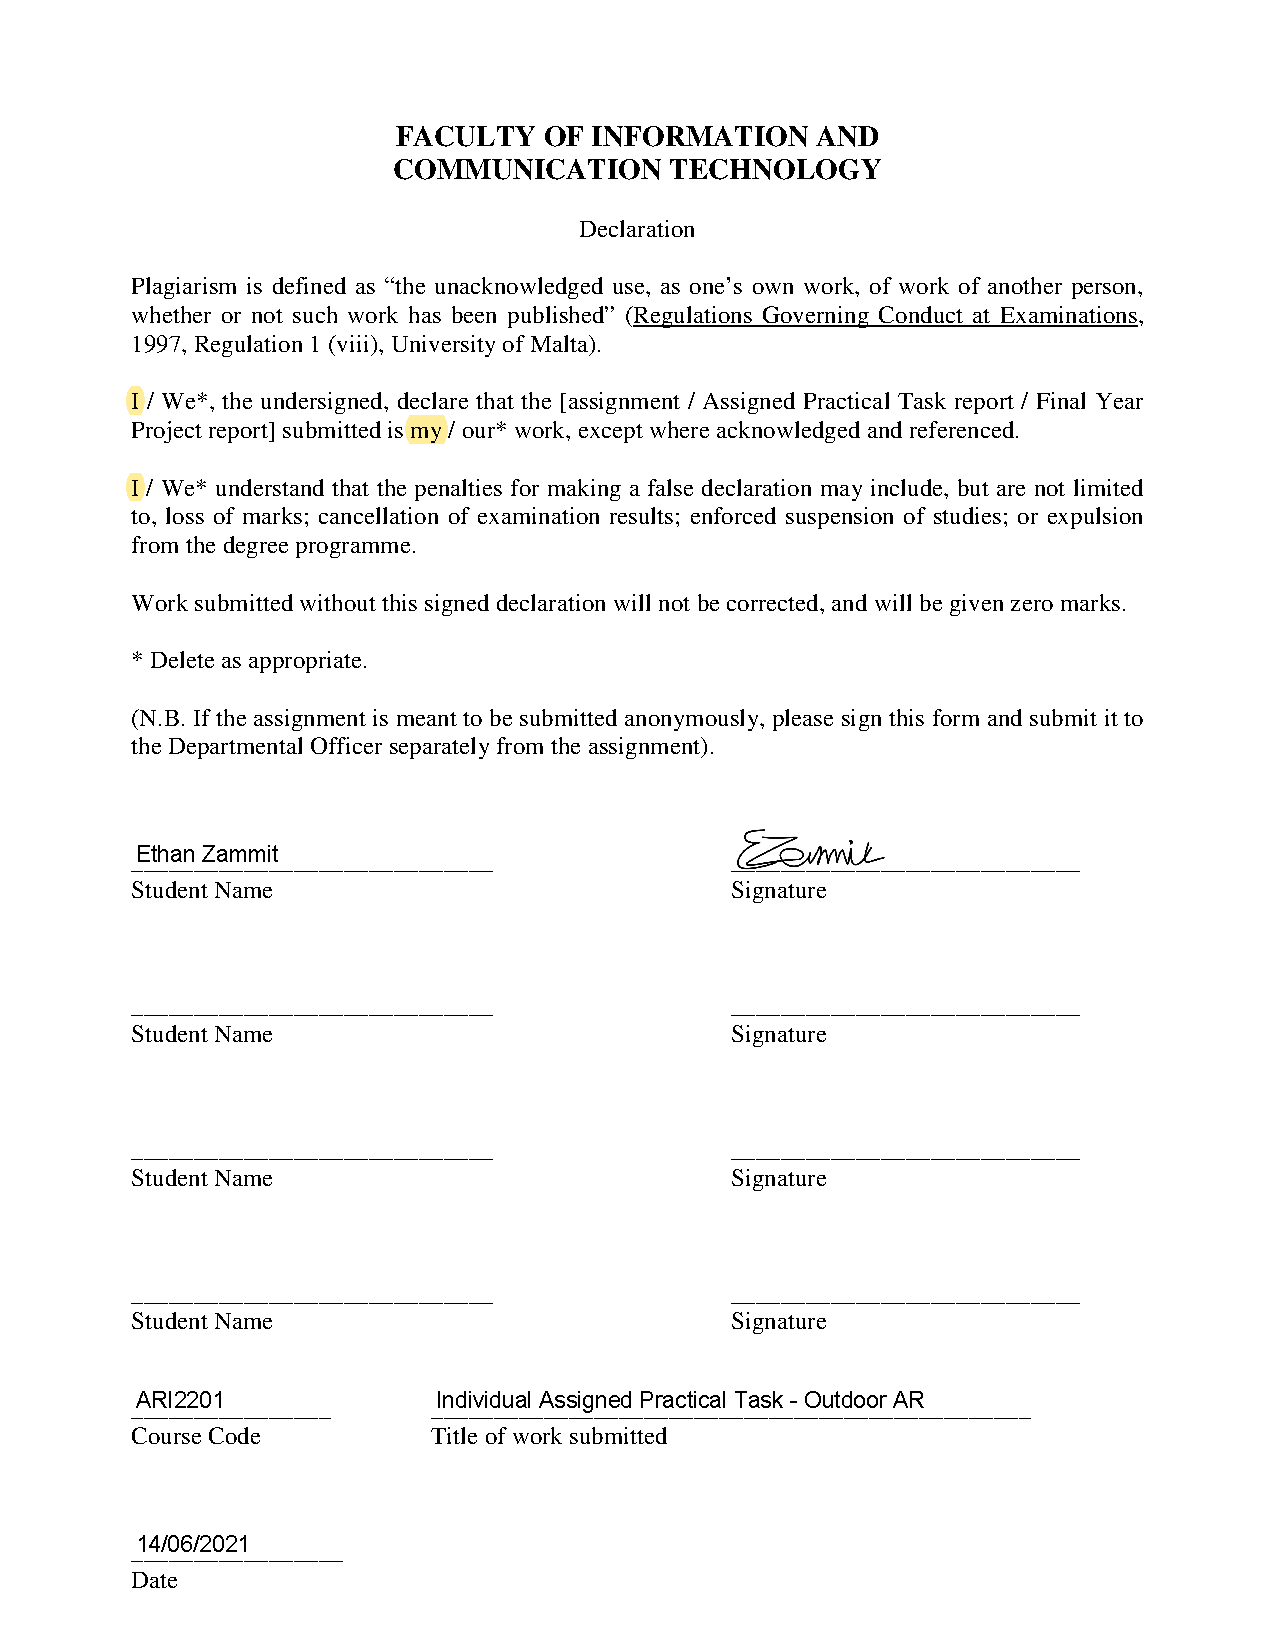
\includepdf[pages={1}]{PlagDecForm.pdf}
\tableofcontents
\pagebreak
%   \begin{IEEEkeywords}
%     OutdoorAR

%   \end{IEEEkeywords}

  \section{Introduction}
    \subsection{Brief of Project}
This project aims to delve into the effects of the exploitation of Augmented Reality Techniques on tourism and heritage.\\
A system is to be developed using Google's ARCore, enabling complex computer vision-based functions to be easily embedded within an andorid app. 
% where users are served an app which enables access to scanning for near landmarks. If the user is within a geofence of a landmark, 
% the user is able to access an Augmented Reality Mode, where the feed of a camera is shown with an overlayed panel, showing information and Images about the site nearby.
\subsection{Aims \& Objectives}
% The main objectove of this project is to explore the technologies available, their feasibility, and the potential effects in the context of tourism. 
% A main focus of this project is also to analyse AR's potential to enable and incentivise tourists to identify and visit heritage sites, 
% whilst also easing the delivery of information in a fun and engaging way, perhaps
% giving a better context about what a site has to offer, and why it's even considered important to begin with.\\
% If well documented, the ability to be provide a tangable experience to otherwise non-tangable sites. Perhaps sites which have been
% lost in wars or disasters. Giving a realistic experience of what a heritage site used to look when it was still in operation. 
There are three main objectives to this project, which are to be explored and implemented to analyse the effects of their combination. 
Firstly,  Augmented Reality is to be used and implemented in the setting of an outdoor environment, using several technologies provided by ARCore,
we may explore different ways that this can be exploited for the best experience. This may even be combined with other sensory data such 
as the location for a better touch with reality. Secondly, an android application is to be developed, which will allow ease of use by most people, avoiding hurdles of 
installations and such. This application is to provide some method of direction to landmarks, and also incorporate the AR experience when 
appropriate. The application is to get information from a server, which will allow for a centralised and controlled method of managing 
landmarks, descriptions and their locations.   

\subsection{Functionality Developed}
\subsubsection{The Application}
An android app was developed that the users can easily install and access. The app constantly uses the location service to consult the API server, providing the device's current
 location and retrieving a list of explorable landmarks. These landmarks are displayed on the application, as a list of potentially explorable landmarks,
  also giving a general bearing of where the 4user should head to reach the site.\\
 When the user is within a (relatively small) proximity of a landmark (geofence defined server-side), the app enables a landmark to be selectable, which when selected, the device enters an AR mode.\\
 When in AR mode, the user can get a floating 3D informational window that contains details about the landmark selected.
 \subsubsection{The API Server}
 The server is to contain a list of landmarks, including their names, locations, a description and maybe even a set of images. The server should allow a device to consult it with
 location-based information and a list of landmarks (within some proximity) is returned to the device, where the device uses the information given and lists them as potential landmarks to explore.\\
 The landmark information is to be stored on the server, so anything can be easily changed by changing the configurations of the server, and the mobile apps simply obtain newer information, 
 without needing to rebuild or update the applications. As this technology may be adopted to other uses, such as games, it would be really useful to be able to have an idea of where 
 players are.

    \section{Background Research}
      \subsection{Location Data \&  Augmented Reality}
In modern smartphones the GPS system is fast and accurate, especially for purposes of landmark geofencing, 
as utmost accuracy is not a requirement. The advancment in smartphone technologies also enable richer AR experiences, as higher quality 
experiences may be included with less concern with device processing power.\\
When these two technologies are combined, the epxerience is taken to another level, as the Augmented Reality experience can shift based on 
the device's real conditiorns and positioning. A level of immersion is reached, as users need to actually move and visit ehritage sites in 
order to experience the Augmented Reality effects, and in return they gain context and heritage information about the landmarks visited.   
\subsection{Google ARCore \& Unity Technologies}
Google ARCore framework greatky facilitates the implementatoon of AR experiences, without the need of reinventing everything from scratch. 
This enables lower-cost projects, lower-qaulified developers and faster integration of AR projects, 
providing a gateway to the mainstream acceptance of AR.\\
Unity 3D technologies combined with Google ARCore enhance the usability of ARCore, as developrs are enabled to keep using existing, 
familiar tools to develop an Augmented Reality Experience. 
\subsection{Augmented Reality \& Tourism}
Augmented Reality has seen it's success in the it industry as can be seen in []. However, according to [] in 2017, the potential of AR
in the tourism domain is still not explored anough, and thus the envolope is still to be pushed for further integration.
    
  % \pagebreak
  \section{Implementation Details}
    \label{Design}
    
\subsection{The Server}
An api server was written in python, as due to the small scale of the application, this was ideal to meet the requirements whilst keeping the 
implementation simple enough. The server provides several endpoints which may be pinged, but only two particular endpoints are used. 
\subsubsection{Location Updates}
The server keeps track of a list of active devices, (though a unique identifier provided on requests), and their last known location.
The device regularly updates the sever wit lcoation infromation, and then requests nearby landmark data. 
The server loops through all landmarks, and calculates the distance between the device longitude and latitude positioning, and the landmark.
If the distance is below some threshold, it is added to a list of potnetially explorable landmarks, which is returned as a JSON response 
to the device. Each landmark entry also contains a geofence region, which when is larger than the distance, the landmarks is considered near 
the user, and the device can knmow that the AR mode can be enabled.
\subsection{The Application}
\subsubsection{Location Service}
On the device, the location is updated every second, with an intended accuracy of 0.1 metres 
(usually not met, but we try to be as accurate as possible).\\
The integrated unity function is used, and a listener is used to check for updates, which update the server,
and the landmarks list accordingly.
\subsubsection{Close Landmark Menu}
A scrollable list was used to show a list of the landmarks returned by the server. The title,
a short description, the raw distance from the location and the bearing to the location is shown for each entry,
 so the user may have some basic information on how to reach a target.
  Whenever the landmarks is very close, the entry become interactable, and the user can press it 
to enter AR mode near the landmark. 
\subsubsection{Augmented Reality Mode}
In this mode, the camera is shown to the user, and a 3D transluscnet floating window is spawned in 3D space.
The user may move around the panel, and observe the panel stays locked in 3D space. The panel shows
some deeper description about the near landmark. A carousel allows the userto see some images of the place
 (as provided through the API).  


\subsection{Main Algortihms}
% The main algorithms used deal with the positioning and distance calculations of the device.
\subsubsection{AR Camera and Pose Driver}
When combined with unity, ARCore gives the developer access to the AR camera and the pose driver, which are responsible for synchronizing movements 
carried out in real life, with the movement inside the game engine. A system is used where 1 unit in the unity engine corresponds to one meter of scale when 
viewed in AR mode. Thus If we need to create a 30cm box, we can just set the size in the engine to 0.3, without needing to do any manual conversion, etc.
\subsubsection{Geometric Distance \& Geofencing}
\subsubsection{Geometric Bearing}


 \subsection{Other AR Techniques}
 A couple of other Augmented Reality techniques were explored during the development of this app. 
 These tecniques were implemented and worked really well as sandalone, yet when combining the features 
 the standalone applications do not have an yuses, and thus there is no way of using them. 
 \subsubsection{Plane detection}
 Although raw plane detection was not used in the final version, under the hood google uses it to keep the 
 floating infromation panel in place. Through goggle's AR Core it is made possible to detect vertical 
 and horizontal planes, to which other game opbjects can be anchored to!\\

 In an example, plane detection was used to find a stable surface, and when the user clicks on a 
 plane, a 3D Game model is spawned in place, and anchored to the plabe. The user is also to walk around 
 in the room, whilst the objects stays anchored to plane! 

 \subsubsection{Image Recognition \& Augmented Images}
 Image Recognition was also a really interesting feature to use. 
 In this projects case, a quick database manager was created in which a list of images could
  be inserted. And actions would be taken according to the image detected!\\

In an example, an image of the earth was used as a key, and when this image is detected, a 3D spinning 
globe would be overlayed on it, where the user is able to go around the globe!
This may have been abnle to implemented in the app, yet as the landmark menu and the ARMode switching 
works, It did not have much room to be used. (As in the near landmark menu, there is 
not access to the camera), and the user may only use AR Mode when near a landmark. However, this 
feature is also fully working, and may easily be implemented if a better use is identified. 



    % \pagebreak
  \section{Evaluation \& Analysis}
  \label{Evaluation}
    
\subsection{Test Analysis}

\subsubsection{Landmark Menu}
The solution as an application was very stable in general, since unity was used, any changes can be done directly through the unity editor, and the benefits of being a 
unity-based application are retained. The aim to provide some sense of direction to the user was also satisfied, as when the GPS connection was established, distance 
and bearing data was accurate. When the GPS connection was unstable, the bearing direction and distance were a little off, yet immediately normalized when the connection was restored. 
\subsubsection{AR Mode}
In general, when discernable plane features are present, the panel stays fixed in place as intended.
Unfortunately, plane detection by design struggles when there are no close discernable attributes (the floor has a regular pattern for example) and there is not much which can be done to 
counteract this issue. The tests performed have also shown that in rare cases, this affects the stability of the position of the panel. However, this does not occur very often, and the 
general experience rarely suffers.
\subsubsection{Server Communication}
Through using the application, the server was also being tested. The solution developed was very responsive, and provided very quick and usable results. 
Distance calculation and geofencing also worked punctually, and the device's locations were updated in real-time.\\
As expandability was also in mind, it is really easy to add, remove and change landmarks, as a simple JSON file is provided, where every bit of detail can be changed.\\
Due to the centralised nature of the application, an internet connection needs to be maintained for most features to work, 
as all landmark information is obtained from the server.
\subsubsection{Critical Analysis}
The few tests performed show that the technologies used are very applicable to the aims and objectives. The strengths of the application match up with the strengths of AR as a concept, 
providing a deep sense of immersion whilst also being informative. On the other hand, the weaknesses of the application are also in sync with the limitations of the concepts by design. Particularly, the application suffers where a stable 
plane is not detected and a plane with lower certainty has to be used, which may cause the information panel to shift positions unexpectedly. 

\subsection{Potential Further Testing}
Three key points mentioned in \cite{Samini2017} have great potential in giving a more formal understanding of the performance of such systems. 
\subsubsection{Variation of Independant Variables}
The feedback provided after variation of independent variables can be used as a performance metric and help analyse the experience of the user, these variables include things that are not 
varied by the user during the test. Examples of such variables include the device size and the field of view of a device's 
camera, which can help conclude the applicability of the technologies adopted with the devices used.
\subsubsection{Variation of Dependent Variables}
The variation of these variables gives a robust metric of how the users react to the 
application presented, such as the number of attempts taken to carry out an action.
Yet this is very application-specific and does not allow much room for comparison between other systems, as 
tasks in an application usually are specific to it.

\subsubsection{Questionnaires}
Questionnaires were mentioned as another performance metric, in contrast to the other tests, this metric is purely subjective. 
In applications such as the tourism domain, this is of utmost importance, as it follows that 
from the user-centric nature, the ultimate goal is to maximise the users' resultant experience, and thus feedback directly from the users may be key.  

% \subsection{Future Works}
% The system was developed with expandability in mind, and thus, it is really easy to adapt the system into different uses cases.
\subsection{Possible Improvements}
\subsubsection{Augmented Images}
Ideally, the augmented imaging feature mentioned in appendix 1 is implemented as another landmark type, as it would allow for a wider range of applications and immersion.
This application would also be applicable in places such as inside museums where for example it would enhance a painting, or have some animation overlayed on it.
\noindent
Another possible improvement is to give better direction towards landmarks, the current application simply gives baring direction and straight line distance between points,
 without any consideration for the streets/obstacles.
\subsection{Future Work}
During development, it was made sure to keep the system as open as possible. Through the 
centralised API, unity engine and other technologies used, the system is meant to be dynamic and 
expandable.\\
With minimal effort, it can be easily be adapted to different uses such as an AR game, 
using google APIs for international standardized locations or even showing 3D models in AR mode. 



  \section{Conclusion}
  \label{Conclusion}
    From the results obtained, through the combination of different technologies, AR provides deep potential when applied to tourism, 
whilst the libraries allow for easier and a more mainstream adaption of the technologies. The effects of location and compass sensory data have 
also been observed to enhance the AR experience even more. Finally, the centralised nature of the server proves for greater expandability and allows 
for data to be changed and reflected in the application in real-time. 

Overall, I managed to meet the intended aims and objectives, and during the process also 
obtained hands-on experience of using the latest technologies to apply the theories learnt into 
practice. Augmented Reality and computer vision as a domain also turned out to be extremely rewarding, as the effort done is immediately reflected in tangible progress. 



  \pagebreak
  \bibliographystyle{IEEEtran}
  \bibliography{IAPTReferences}

  \pagebreak
  \section{Appendices}
  \label{Appendices}
  % \section{}
\pagebreak
 \section*{Appendix 1 - Image Recognition \& Augmentation}
 Image Recognition was also a really interesting feature to use, yet unfortunately, it is not used in the application. This may have been able to be implemented, yet with the current implementations 
 of the landmark menu and the ARMode switching, It did not make much sense to be used. (As in the near landmark menu, there is no access to the camera), and the user may only use AR Mode when near a landmark.\\
 However, this feature is also fully working, and may easily be implemented if a better use in the context of outdoor AR is identified. 
 In the case of this project, a quick database manager was created in which a list of images could
  be inserted. These images also need to have specific features, to be distinguishable from other places (for example some image of plain grey gravel is not very easily distinguishable, 
  but an image of the earth is). And actions would be taken according to the image detected!
  \subsubsection*{Testing}
As augmented images were implemented some basic testing was also involved, where a simple image of the earth was detected, and overlayed with a 3D spinning globe. 
The image was recognized from different angles and light settings whilst tracking also was really responsive to even moving the image.
\begin{figure}[!htb]
    \minipage{0.4\textwidth}
        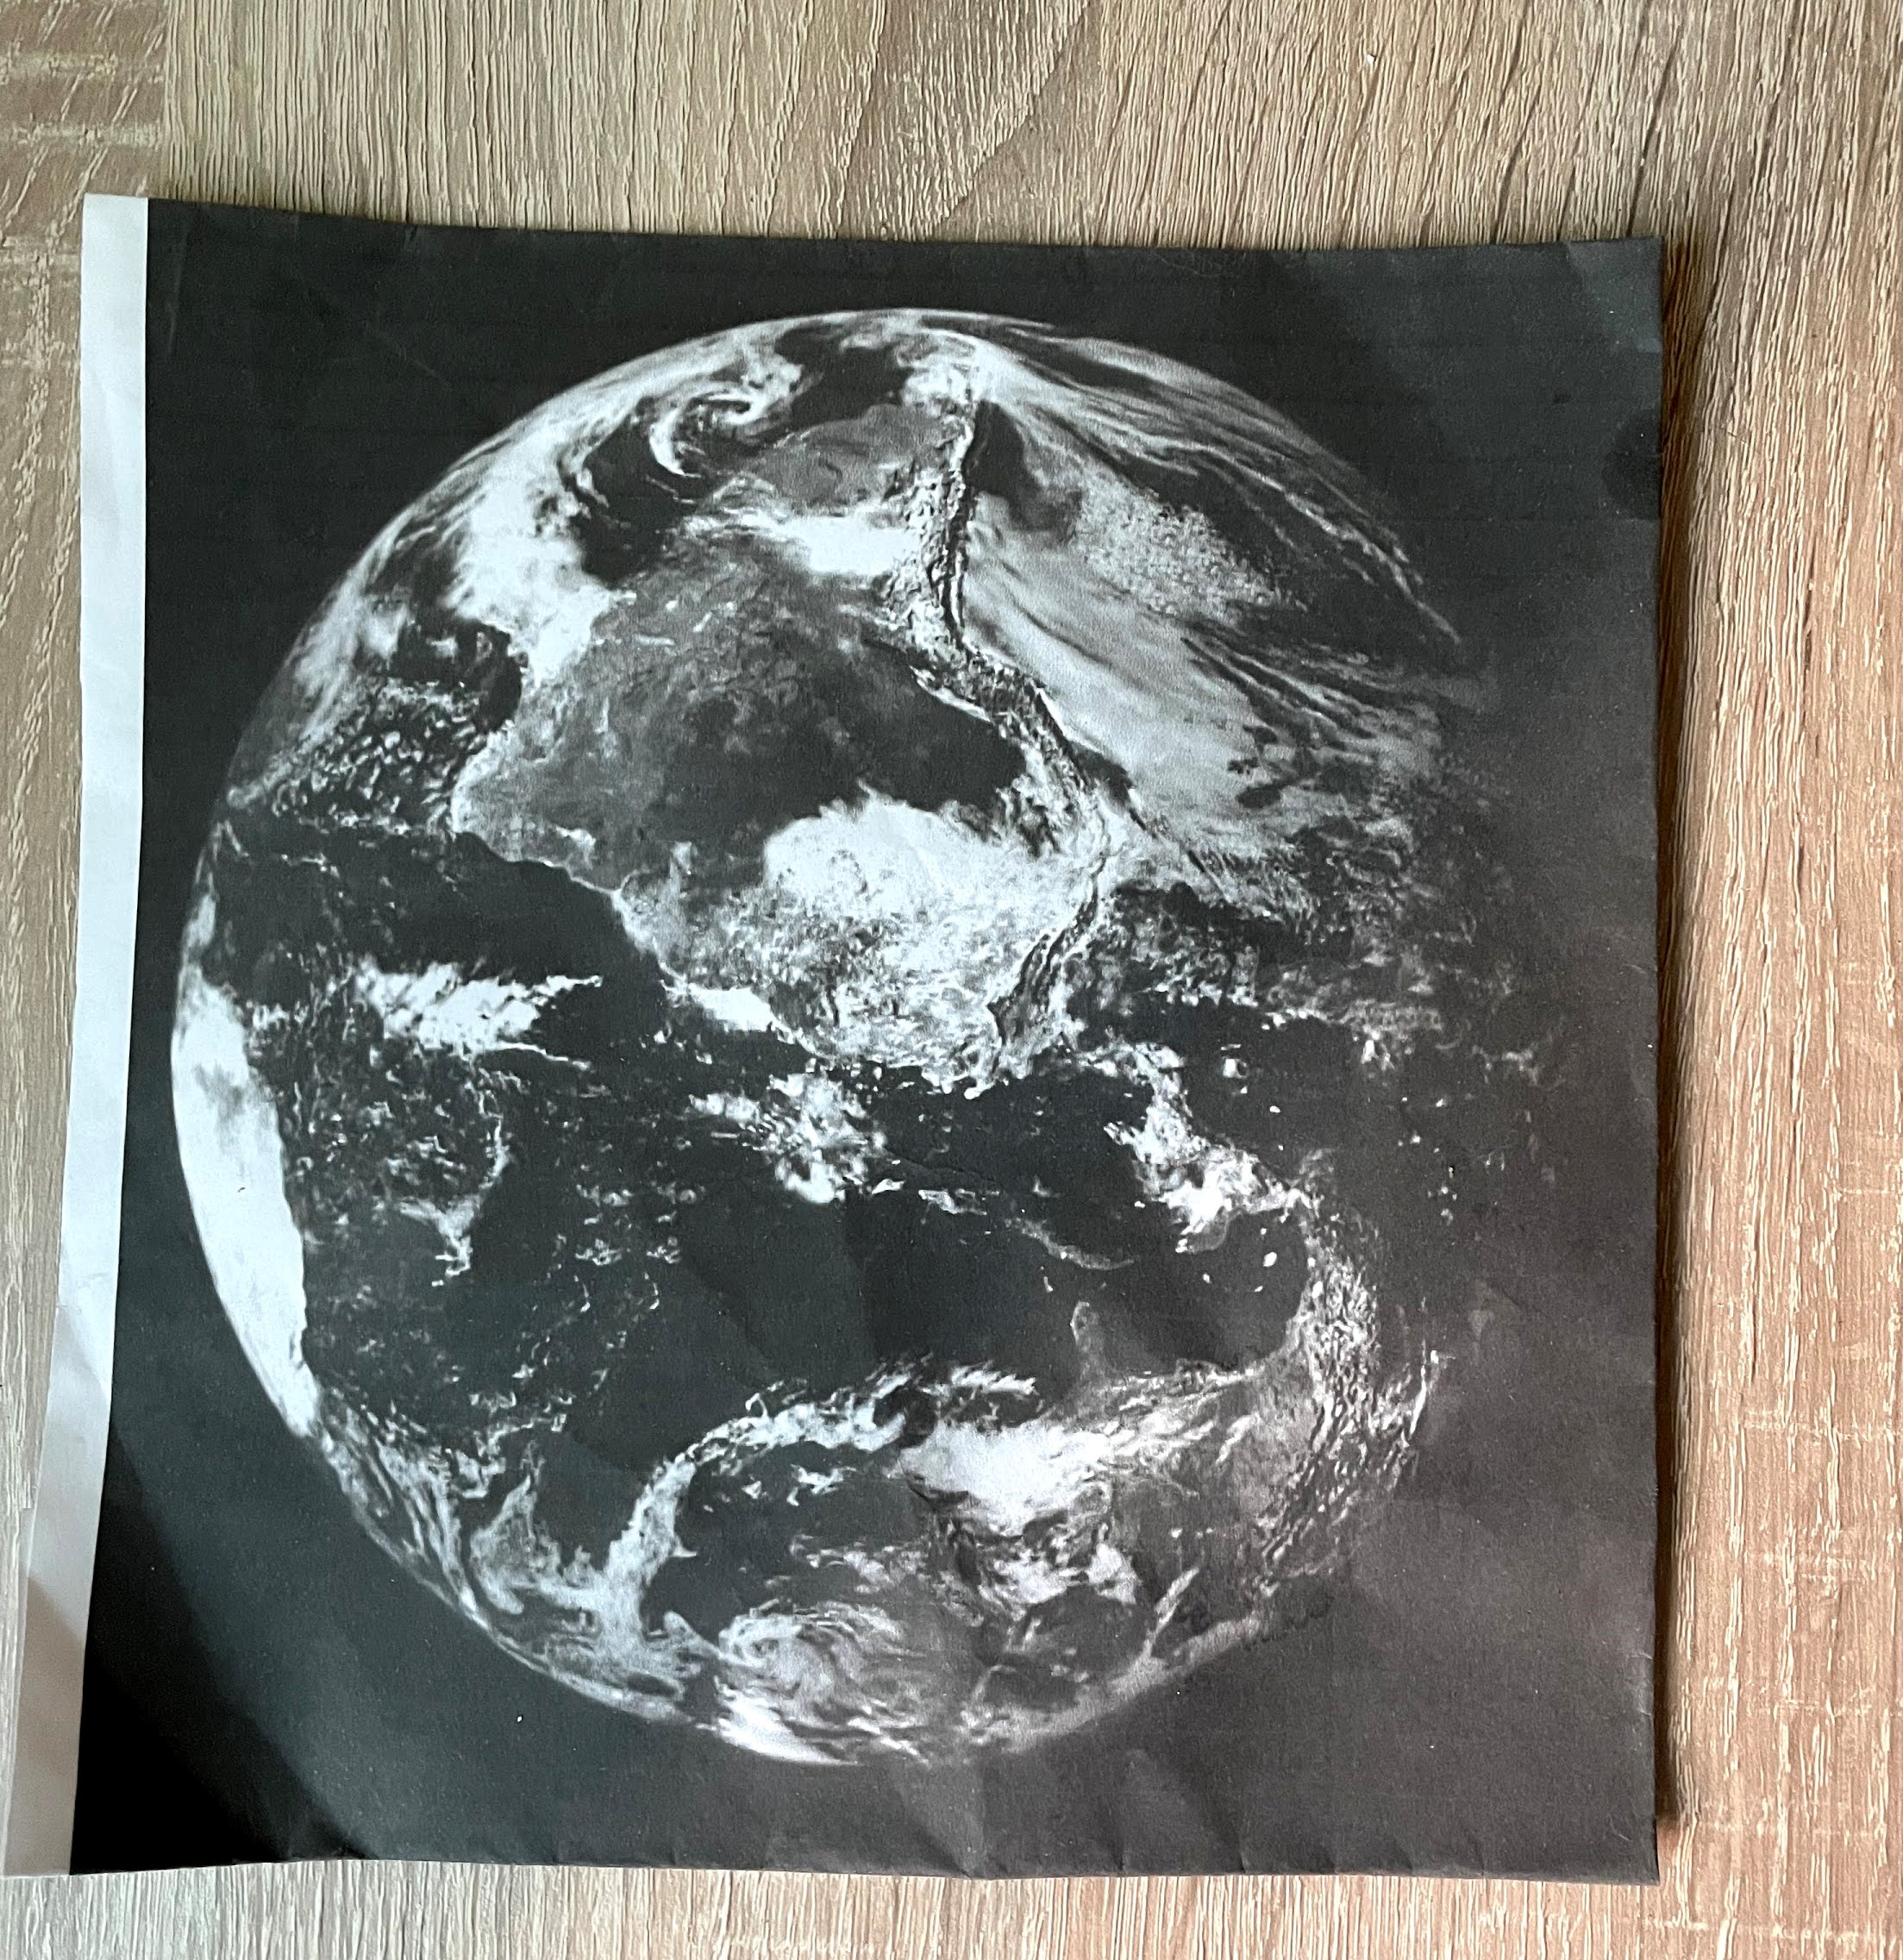
\includegraphics[width=\linewidth]{earth_og}
            \caption{Earth Image Key}
            \label{fig:earth_og}
    \endminipage\hfill
    \minipage{0.4\textwidth}
        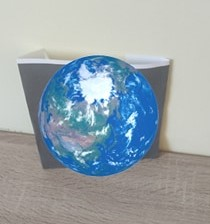
\includegraphics[width=\linewidth]{earth_ov}
        \caption{3D sphere overlayed}
        \label{fig:earth_ov}
    \endminipage
    \end{figure}

\end{document}